\documentclass{article}
\usepackage[francais]{babel}
\usepackage[utf8]{inputenc}
\usepackage{xcolor}
\usepackage[pdftex]{graphicx}
\usepackage{listings}
\usepackage{amsmath}
\usepackage[a4paper,includeheadfoot,margin=2.54cm]{geometry}
\usepackage{amsfonts}
\usepackage{fancyhdr}
\usepackage{titling}
\usepackage{algorithm}
\usepackage{algpseudocode}
\usepackage{hyperref}

\pagestyle{fancy}
\fancyhf{}
\fancyhead[LE,RO]{\theauthor}
\fancyhead[RE,LO]{\thetitle}
\fancyfoot[CE,CO]{\leftmark}
\fancyfoot[LE,RO]{\thepage}

\usepackage[thinlines]{easytable}

\title{Atelier d'approfondissement en informatique: Graphes et Algorithmes}
\author{Quentin Garrido}
\date{21 avril 2019}

\begin{document}

\maketitle
\tableofcontents
\pagebreak

%=============================================================================%
\section{Introduction}
\subsection{Objectifs}

L'objectif de ce projet est d'implémenter des algorithmes de recherche de plus courts
chemins dans un graphe, et plus particulièrement dans un graphe représentant le réseau
de métro de Paris.\\
Nous implémenterons tout d'abord l'algorithme de Dijkstra, puis le modifierons pour
qu'il utilise la stratégie  A* et nous optimiserons son temps d'éxécution grâce
à des structures de données adaptées.

\subsection{Utilisation}

Tout le code source est disponible à l'adresse suivante: \textit{https://github.com/garridoq/metro-shortest-path}.\\

Tout les éxécutables devraient vous être fournis dans le mail et devraient fonctionner sans devoir
les recompiler. Dans le cas contraire voici la démarche à suivre:\\

Un makefile est fourni pour la compilation, il servira à compiler les bibliothèques et les tests.
Une fois le code source obtenu il faudra exécuter la commande suivante pour compiler les bibliothèques:
\begin{lstlisting}[language=bash]
	> make
\end{lstlisting}

Vous pourrez alors compiler tous les fichiers de tests de la manière suivante:
\begin{lstlisting}[language=bash]
	> make NOM.exe
\end{lstlisting}
Où NOM est le nom du fichier de test (pour test\_heap.c, il faudra entrer make test\_heap.exe).\\

Voici la liste des fichiers de test et leur utilisation:
\begin{itemize}
	\item test\_heap:./test\_heap.exe , ce fichier permet de tester l'implémentation du tas
		  binaire et de ses opérations primaires.
	\item test\_dijkstra:./test\_dijkstra.exe GRAPH DEBUT FIN , ce fichier va récupérer
		  le graphe dans le fichier GRAPH, puis calculer le plus court chemin de DEBUT à FIN
		  en utilisant l'agorithme de Dijkstra, l'A* et A* avec une file de priorité.\\
		  Un fichier EPS sera créé pour chaque algorithme.\\
\end{itemize}

Afin de trouver le numéro de station associé à un nom vous pouvez utiliser la commande suivante:
\begin{lstlisting}[language=bash]
	> cat GRAPHE | grep -iF NOM
\end{lstlisting}
La recherche n'est pas sensible à la casse mais l'est aux accents. Vous obtiendrez alors
toutes les stations contenant NOM et leur numéro associé.\\

À titre de référence, voici sur la filgure~\ref{metro} à quoi ressemble le graphe entier du réseau de métro, que nous
utiliserons par la suite:\\
Les stations sont réprésentées par les sommets et nous avons une arc entre deux sommets
si ils sont reliés par le métro.

\begin{figure}[!hbt]
	\centering
	\includegraphics[width=\textwidth]{metro.eps}
	\caption{Graphe de référence du métro}
	\label{metro}
\end{figure}


\clearpage
%=============================================================================%
\section{Calcul du symmétrique}
\subsection{Première version}

Voici la première version de l'algorithme pour calculer le symmétrique d'un graphe (algorithme fourni):

\begin{algorithm}
\caption{Calcul de symmétrique 1}\label{sym1}
\begin{algorithmic}[1]
\Procedure{Sym1}{$E, \Gamma$}
	
	\ForAll{$x \in E$}
		\State $\Gamma^{-1} = \emptyset$
	\EndFor
		
	\ForAll{$x \in E$}
		\ForAll{$y \in E$}
			\If{$y \in \Gamma(x)$}
				\State $\Gamma^{-1}(y) = \Gamma^{-1}(y) \bigcup \{x\}$
			\EndIf
		\EndFor
	\EndFor
	
		\State \textbf{return} $\Gamma^{-1}$
\EndProcedure
\end{algorithmic}
\end{algorithm}

Cet algorithme est en $O(n + n\times n \times n) = O(n^3)$.\\
Nous pouvons voir que cette version n'est pas efficace car nous regardons pour tous les sommets si
ils sont des successeurs de $x$, ce qui est un test redondant étant donné que $\Gamma$ est fournie,
nous pouvons directement obtenir les successeurs de $x$.

\subsection{Version améliorée}

En parcourant directement tous les successeurs de $x$ nous obtenons l'algorithme suivant:

\begin{algorithm}
\caption{Calcul de symmétrique 2}\label{sym2}
\begin{algorithmic}[1]
\Procedure{Sym2}{$E, \Gamma$}
	
	\ForAll{$x \in E$}
		\State $\Gamma^{-1} = \emptyset$
	\EndFor
		
	\ForAll{$x \in E$}
		\ForAll{$y \in \Gamma(x)$}
			\State $\Gamma^{-1}(y) = \Gamma^{-1}(y) \bigcup \{x\}$
		\EndFor
	\EndFor
	
		\State \textbf{return} $\Gamma^{-1}$
\EndProcedure
\end{algorithmic}
\end{algorithm}

La complexité de l'algorithme est désormais $O(n + m)$. Puisque $m < n^2$ nous pouvons être sûrs que 
cette version sera toujours plus rapide que la précédente, voici des comparaisons des temps d'éxécution
sur des graphes de tailles différentes:\\


\begin{center}
\begin{tabular}{| c | c | c | c | c |}
	\hline
	 Sommets & Arcs & Temps avec Sym1 (en $\mu s$)& Temps avec Sym2(en $\mu s$) & rapport \\ \hline
	 100 & 500 & 150 & 20 & 7,5 \\ \hline
	 100 & 4000 & 1000 & 350 & 2.78\\ \hline
	 500 & 20000 & 29000 & 1800 & 16.11 \\ \hline
	 500 & 120000 & 235000 & 73000 & 3.22 \\ \hline
\end{tabular}
\end{center}

Comme nous pouvons la deuxième version est bien plus rapide que la première, d'autant plus lorsque
$m << n^2$ et même quand $m$ se rapproche de $n^2$ nous sommes toujours bien plus rapide.\\
Nous utiliserons donc cette deuxième version par la suire lorsque nous en aurons besoin.

\clearpage
%=============================================================================%
\section{Algorithme de Dijkstra}
\subsection{Implémentation}

Pour calculer le chemin le plus court d'un point D à A nous allons utiliser 
la version suivante de l'algorithme de Dijkstra, adaptée depuis le cours de 
l'unité Graphes et Algorithmes.\\

Ici nous n'avons pas besoin de calculer les chemins de notre sommet de départ
vers tous les autres sommets du graphe et nous nous arrêterons donc dès
que nous atteignons notre sommet d'arrivée.

\begin{algorithm}
\caption{Algorithme de Dijkstra}\label{dijkstra}
\begin{algorithmic}[1]
\Procedure{DIJKSTRA}{$E, \Gamma, l, d \in E, a \in E$}
	\State S = \{d\}, $\pi(d)$ = 0, k = 1, $x_1$ = d
	\ForAll{$x \in E$\textbackslash$ \{d\}$}
		\State $\pi(x) = \infty$
	\EndFor
	
	\While{$k < n$ et $\pi(x_k) < \infty$ }
		\ForAll{$y \in \Gamma(x_k) $ tel que $y \not\in S$}
			\State $\pi(y) = $ min[$\pi(y), \pi(x_k) + l(x_k, y)$]
		\EndFor
		\State Extraire $x \not\in S$ tel que $\pi(x)$=min$\{\pi(y), y \not\in S\}$
		\State k = k + 1, $x_k = x$, S = S $\bigcup \{x_k\}$
		\If{$x_k = a$}
			\State \textbf{break}
		\EndIf
	\EndWhile
	
	\State \textbf{return} $\pi$, S
\EndProcedure
\end{algorithmic}
\end{algorithm}

Nous implémentons S avec un tableau de $n = \vert E\vert$ éléments, correspondants aux sommets 
de notre graphe.\\
Ainsi nous l'initialiserons entièrement à 0 et S = S $\bigcup \{x_k\}$
correspondra à faire S[k] = 1.\\
Bien que cette implémentation soit plus coûteuse en mémoire qu'une liste chaînée
elle permettra d'implémenter l'appartenance à S en temps constant, opération très
utilisée aux lignes 7 et 10.\\
De plus l'ajout d'un élément sera aussi simplifié car nous n'aurons pas à vérifier
l'appartenance avant de l'insérer ou non.\\

\subsection{Récupération du plus court chemin}


Soit $c$ notre chemin de coût minimum, pour tout $u = (x,y) \in \vec{\Gamma}$, $ u \in c$ si 
$l(x,y) = \pi (y) - \pi (x)$ avec $\pi(x)$ le coût d'un plus court chemin de $i$ (notre point de départ)
à $x$.\\

Nous allons donc utiliser cette propriété pour trouver notre plus court chemin grâce à
l'algorithme suivant :\\

\clearpage


\begin{algorithm}
\caption{Plus court chemin}\label{pcc}
\begin{algorithmic}[1]
\Procedure{PCC}{$\pi, \Gamma^{-1}, l, d \in E, a \in E$}
	\State x = a, c = $\emptyset$
	\While{$x \neq d$}
		\ForAll{$y \in \Gamma^{-1}(x)$}
			\If{$\pi (x) - \pi (y) =  l(y, x)$}
				\State $c = c \bigcup \{(y,x)\}$
				\State x = y
				\State \textbf{break}
			\EndIf
		\EndFor
	\EndWhile
	
	\State \textbf{return} c
\EndProcedure
\end{algorithmic}
\end{algorithm}

\subsection{Résultats}

Considérons un trajets des stations Alexandre Dumas (1) à Porte Dauphine (256).
Nous trouvons alors le chemin le plus court suivant:\\

Alexandre Dumas
$->$ Philippe-Auguste
$->$ Père Lachaise
$->$ Ménilmontant
$->$ Couronnes
$->$ Belleville
$->$ Colonel Fabien
$->$ Jaurès
$->$ Stalingrad
$->$ La Chapelle
$->$ Barbès Rochechouart
$->$ Anvers
$->$ Pigalle
$->$ Blanche
$->$ Place de Clichy
$->$ Rome
$->$ Villiers
$->$ Monceau
$->$ Courcelles
$->$ Ternes
$->$ Charles de Gaulle, Étoile
$->$ Victor Hugo
$->$ Porte Dauphine\\

Nous pouvons observer ce chemin sur la figure~\ref{dijkstra_1}. Les arcs forment le plus court
chemin et les sommets sont uniquement ceux visités. Nous en avons visité 329 sur 376.\\

\begin{figure}[!hbt]
	\centering
		\includegraphics[width=0.7\textwidth]{dijkstra_1_256.eps}
	\caption{Résultat de l'algorithme de Dijkstra pour aller des sommets 1 à 256}
	\label{dijkstra_1}
\end{figure}

Comme nous pouvons le voir nous avons parcouru des sommets qui nous éloignaient grandement du résultat
uniquement car le coût pour y aller était plus faible (cf ligne 10 de l'algorithme).\\
Cet effet est exacerbé ici car le trajet que nous avons choisi est particulièrement long.\\
Ce constat reste le même sur tous les trajets, sauf sur ceux très courts.\\

Bien que le chemin que nous trouvions ne paraisse pas optimal, nous l'avons vérifié via
le service Vianavigo de la RATP, où nous trouvons le même chemin. Cela est dû au fait que
les deux stations sont sur la même ligne et donc que nous avons aucun changement à faire,
d'où la plus courte durée du trajet.\\\\
Nous avons vérifié plusieurs autres trajets de la même manière avec le même résultat à chaque
fois, ainsi notre implémentation semble être correcte, à condition que l'algorithme
utilisé par la RATP pour Vianavigo soit correct, ce que nous pouvons affirmer être vrai.

\pagebreak
%=============================================================================%
\section{Stratégie A*}

Pour utiliser la stratégie A* nous allons appliquer une heuristique lors du choix du prochain
sommet à étudier dans l'algorithme de Dijkstra, ce qui correspond à la ligne 10 de l'algorithme.\\
En effet nous avons pu voir que choisir toujours le somemt avec le plus court chemin vers lui
se révèle sous optimal car nous allons partir dans des directions qui nous éloignent de l'arrivée.\\
Nous allons donc essayer de choisir une heuristique qui va nous permettre d'explorer moins de sommets.\\

Le principe de la stratégie A* est le suivant:\\
On considère $f(n)$ une estimation du  coût d'un plus court chemin de notre départ $d$ à notre arrviée $a$ passant par n.
On a alors:
\begin{gather*}
		f(n) = g(n) + h(n)
\end{gather*}
g(n) est le coût d'un chemin optimal de $d$ à $n$, dans notre cas $\pi(n)$.\\
h(n) est notre heuristique qui estimera le coût d'un chemin optimal de $n$ à $a$.\\

Nous utiliserons alors cette fonction $f$ pour comparer deux sommet et savoir lequel
nous allons étudier ensuite.

\subsection{Choix de l'heuristique}

Dans notre cas, la durée de trajet entre deux stations correspond au poids de l'arc. Cette valeur
est calculée pour un métro se déplaçant en moyenne à 10 $m.s^{-1}$ et une unité dans notre graphe
correspond à 25.7 m.\\

L'heuristique que nous devons choisir doit estimer le plus court chemin du sommet courant à l'arrivée.
Ainsi nous allons utiliser la distance euclidienne entre notre sommet actuel et l'arrivée.\\
Nous possédons les coordonnées de tous les sommet mais il faut les convertir en mètres en multipliant
par 25.7 puis diviser par 10 pour obtenir une valeur comparable aux valeurs des arcs, et par 
conséquent des longueurs de chemins.\\
Cette heuristique devrait s'avérer bonne car très simple à calculer et elle représente le trajet à
vol d'oiseau entre nos stations, ce qui est le résultat optimal peu importe le moyen de transport
utilisé, aucun trajet ne peut être plus court que cela.\\

Notre heuristique est alors:

\begin{algorithm}
\caption{Heuristique}\label{heuristique}
\begin{algorithmic}[1]
\Procedure{heuristique}{$E,i \in E, a \in E$} \Comment{a est notre point d'arrivée}
	\State \textbf{return} distance\_euclidienne(i, a) $\times \frac{25.7}{10}$
\EndProcedure
\end{algorithmic}
\end{algorithm}

Une seule question subsiste, il s'agit de l'optimalité de la solution. En effet si notre heuristique
est trop `forte' par rapport aux valeurs des chemins nous n'explorerons jamais certains sommets
qui nous donneraient un plus court chemin.\\
L'algorithme A* trouvera une solution optimale si l'heuristique est admissible, c'est à dire si
l'heuristique ne surestime jamais le coût pour atteindre l'arrivée.\\
Dans notre cas, la distance euclidienne étant toujours la distance optimale (en supposant que nous sommes
dans un plan, en réalité ce n'est pas le cas à cause de la courbure de la Terre, mais l'approximation
est acceptable dans notre cas, Paris n'étant pas assez vaste pour que la courbure aie une grande influence)
nous pouvons garantir l'optimalité de la solution trouvée.\\\\

Nous pouvons bien voir qu'avec cette condition d'optimalité, l'algorithme de Dijkstra trouve une solution
optimale car il correspond à avoir une heuristique toujours égale à 0, or dans un réseau avec des arcs
à valeur positive, un chemin est toujours plus long que 0.

\subsection{Implémentation de l'algorithme}

Pour implémenter la stratégie A* seules de très légères modifications de l'algorithme de Dijkstra sont
nécessaires, il nous suffit de modifier le choix du prochain sommet à étudier à chaque étape.
Nous obtenons alors:\\

\clearpage


\begin{algorithm}
\caption{Algorithme A*}\label{astar}
\begin{algorithmic}[1]
\Procedure{A*}{$E, \Gamma, l, d \in E, a \in E$}
	\State S = \{d\}, $\pi(d)$ = 0, k = 1, $x_1$ = d
	\ForAll{$x \in E$\textbackslash$ \{d\}$}
		\State $\pi(x) = \infty$
	\EndFor
	
	\While{$k < n$ et $\pi(x_k) < \infty$ }
		\ForAll{$y \in \Gamma(x_k) $ tel que $y \not\in S$}
			\State $\pi(y) = $ min[$\pi(y), \pi(x_k) + l(x_k, y)$]
		\EndFor
		\State Extraire $x \not\in S$ tel que $\pi(x)$=min$\{\pi(y)+$heuristique(y)$, y \not\in S\}$
		\State k = k + 1, $x_k = x$, S = S $\bigcup \{x_k\}$
		\If{$x_k = a$}
			\State \textbf{break}
		\EndIf
	\EndWhile
	
	\State \textbf{return} $\pi$, S
\EndProcedure 
\end{algorithmic}
\end{algorithm}

\subsection{Résultats}

Afin de pouvoir comparer la stratégie A* et Dijkstra de manière la plus juste possible nous allons
réutiliser le même chemin que précédemment.\\

Nous obtenons désormais la figure suivante:\\

\begin{figure}[!hbt]
	\centering
		\includegraphics[width=0.7\textwidth]{as_1_256.eps}
	\caption{Résultat de la stratégie A* pour aller des sommets 1 à 256}
	\label{as_1}
\end{figure}

Comme nous pouvons le voir, nous explorons bien moins de sommet, avec la stratégie A* nous en
explorons uniquement 89 contre 329 auparavant.\\
Cela se traduit au niveau du temps d'éxécution qui passe de 550$\mu s$ à 241$\mu s$ ce qui est
une amélioration très importante, et qui le sera de plus en plus en augmentant la taille du
graphe.
Comme attendu, nous priorisons les sommets nous rapprochant de l'arrivée et donc il ne nous arrive
plus de partir dans des directions opposées. Cet exemple est un des pire cas possible pour 
la stratégie A* dans notre problème car le chemin le plus court est tout sauf direct pour
l'arrivée, ce qui rend moins efficace notre heuristique.\\

Afin de mieux se rendre compte des différences entre nos stratégies voici d'autres exemples
d'éxécution :\\


\begin{figure}[!hbt]
		\begin{minipage}{0.45\textwidth}
			\centering
			\includegraphics[width=0.8\textwidth]{d_130_212.eps}
		\end{minipage}
		\begin{minipage}{0.45\textwidth}
			\centering
			\includegraphics[width=0.8\textwidth]{as_130_212.eps}
		\end{minipage}
		\caption{Comparaison entre Dijkstra(à gauche) et A*(à droite) de 130 à 212}
		\label{vs_1}
\end{figure}


\begin{figure}[!hbt]
		\begin{minipage}{0.45\textwidth}
			\centering
			\includegraphics[width=0.8\textwidth]{d_27_244.eps}
		\end{minipage}
		\begin{minipage}{0.45\textwidth}
			\centering
			\includegraphics[width=0.8\textwidth]{as_27_244.eps}
		\end{minipage}
		\caption{Comparaison entre Dijkstra(à gauche) et A*(à droite) de 27 à 244}
		\label{vs_2}
\end{figure}

\clearpage

\begin{figure}[!hbt]
		\begin{minipage}{0.45\textwidth}
			\centering
			\includegraphics[width=0.8\textwidth]{d_200_201.eps}
		\end{minipage}
		\begin{minipage}{0.45\textwidth}
			\centering
			\includegraphics[width=0.8\textwidth]{as_200_201.eps}
		\end{minipage}
		\caption{Comparaison entre Dijkstra(à gauche) et A*(à droite) de 200 à 201}
		\label{vs_3}
\end{figure}

\begin{figure}[!hbt]
		\begin{minipage}{0.45\textwidth}
			\centering
			\includegraphics[width=0.8\textwidth]{d_146_212.eps}
		\end{minipage}
		\begin{minipage}{0.45\textwidth}
			\centering
			\includegraphics[width=0.8\textwidth]{as_146_212.eps}
		\end{minipage}
		\caption{Comparaison entre Dijkstra(à gauche) et A*(à droite) de 146 à 212}
		\label{vs_3}
\end{figure}


Voici la comparaison des temps d'éxécution sur ces exemples:\\

\begin{center}
\begin{tabular}{| c | c | c | c | c |}
	\hline
	 Départ & Arrivée & Temps avec Dijkstra (en $\mu s$)& Temps avec A*(en $\mu s$) & rapport \\ \hline
	 130 & 212 & 350 & 110 & 3.18 \\ \hline
	 27 & 244 & 500 & 420 & 1.19\\ \hline
	 200 & 201 & 600 & 530 & 1.13 \\ \hline
	 146 & 212 & 230 & 170 & 1.35 \\ \hline
\end{tabular}
\end{center}

Nous pouvons voir que comme sur notre autre exemple nous parcourons en général bien moins de 
sommet mais le temps d'éxécution ne varie pas toujours autant que précédemment.\\
Mais même dans le pire de nos exemples, nous avons quand même un gain de 13\%, ce qui
reste intéressant.

\clearpage
%=============================================================================%
\section{Tas Binaire}

Que ce soit dans l'algorithme de Dijkstra ou dans la stratégie A*, une des opérations les 
plus coûteuses reste la ligne 10, lorsque que nous calculons un minimum, cette opération
s'effectue en $O(n)$.\\
Cependant avec des structures de données adaptées cette opération peut devenir en $O(1)$ (ou
$O(log(n))$ si nous souhaitons extraire ce minimum)
tout en gardant une compléxité en $O(log(n))$ pour les autres opérations. Une des structures
permettant cela est le tas binaire, qui est relativement simple à implémenter.\\

Un tas binaire est un arbre binaire qui possède à sa racine son élément le plus petit (tas minimun) ou
le plus grand (tas maximum).\\
De plus pour chaque noeud dans l'arbre tous ses `enfants' son plus petits que lui (tas minimum) ou
plus grands (tas maximum).


\subsection{Implémentation classique}

Tout d'abord nous avons implémenté un tas binaire sans qu'il serve de file de priorité.\\
Afin de l'implémenter nous avons utilisée un struct contenant un tableau (les éléments),
sa capacité maximale, et sa capacité actuelle.\\
Par la suite nous parlerons uniquement d'un tas binaire minimum car c'est celui ci que 
nous souhaitons utiliser pour notre problème.\\

En effet un tas binaire peut être implémenté avec un tableau uniquement, comme nous
pouvons le voir sur le schéma suivant:

\begin{figure}[!hbt]
		\centering
		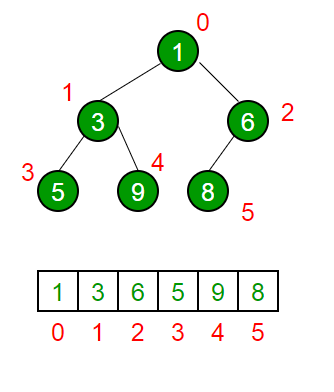
\includegraphics[width=0.5\textwidth]{binaryheap.png}
		\caption{Représentation en mémoire d'un tas binairei - Source: geeksforgeeks.org}
		\label{vs_3}
\end{figure}

Pour chaque noeud (indicé i), nous pouvons obtenir son parent et ses enfants
de la manière suivante:
\begin{itemize}
	\item parent(i)  = $\lfloor \frac{i-1}{2}  \rfloor$
	\item gauche(i) = $i \times 2 + 1$
	\item droite(i) = $i \times 2 + 2 $\\ 
\end{itemize}

Le tas binaire doit supporter les opérations suivantes, dont nos implémentations proviennent de 
\textit{Introduction à l'algorithmique}:
\begin{itemize}
	\item minHeapify(t, i) : cette méthode va rétablir les propriétés du sous tas t à l'indice i
	\item insert(x) : cette méthode va insérer un élément dans notre tas via minHeapify
	\item buildMinHeap(tab) : cette méthode va construire un tas à partir d'un tableau non trié\\
\end{itemize}

Vous pourrez trouver un implémentation d'un tas maximum dans le fichier \textit{heap.c} et 
les tests via le fichier \textit{test\_heap.c}.

\subsection{Implémentation pour notre problème}

Afin de pouvoir utiliser un tas binaire comme file de priorité il va falloir y apporter quelques
modifications liées à notre problème.\\

Nous allons utiliser deux tableaux, \textit{elements} qui contient les sommets de notre graphe
et \textit{keys} qui contient les valeurs utilisées pour le tri dans le tas. Dans \textit{keys} nous
stockerons le coût d'un plus court chemin vers notre sommet plus son heuristique.\\

Un troisième tableau à $n$ éléments, \textit{indice} sera utilisé afin de savoir si un sommet est
déjà présent dans le tas et si il y est où se trouve-t-il, si il est absent nous utiliserons la valeur -1.
Nous avons alors indice[i] = argument de i dans \textit{elements}.\\
Ce tableau nous permettra de savoir si un sommet est dans le tas binaire en temps constant,
ce qui nous sera utile pour savoir si nous allons devoir insérer un sommet ou juste 
mettre sa clef à jour. Nous pourrions toujours réinsérer un sommet peut importe qu'il y soit ou
non mais cela nous forcerait a utiliser un tas de taille maximale dynamique, et aurait aussi
pour conséquence de ralentir l'ajout d'éléments dans la file de priorité car le tas 
contiendrait plus d'éléments.\\

Nous aurons aussi besoin des nouvelles fonctions suivantes:
\begin{itemize}
	\item minInsert(elt, key): il s'agit d'une variante de \textit{insert} qui insère un 
		élément et sa clef associée dans notre file de priorité
	\item getMin(t) : cette fonction retourne l'élément minimum dans la file de priorité (l'élément
		à l'indice 0)
	\item extractMin(t): cette fonction va enlever l'élément minimal de la file de priorité
			et le retourner.
	\item decreaseKey(elt, key): cette fonction va baisser la valeur de la clef de l'élément \textit{elt}
			pour y mettre la valeur \textit{key}. Elle s'effectue en temps logarithmique grâce à notre 
			tableau \textit{indices}\\
\end{itemize}

Nous allons alors modifier notre algorithme pour utiliser cette file de priorité afin d'obtenir
plus rapidement l'élément minimum:

\clearpage

\begin{algorithm}
\caption{Algorithme A* avec file de priorité}\label{astar_pq}
\begin{algorithmic}[1]
\Procedure{A*}{$E, \Gamma, l, d \in E, a \in E$}
	\State S = \{d\}, $\pi(d)$ = 0, k = 1, $x_1$ = d, file = $\emptyset$
	\ForAll{$x \in E$\textbackslash$ \{d\}$}
		\State $\pi(x) = \infty$
	\EndFor
	\While{$k < n$ et $\pi(x_k) < \infty$ }
		\ForAll{$y \in \Gamma(x_k) $ tel que $y \not\in S$}
			\State $\pi(y) = $ min[$\pi(y), \pi(x_k) + l(x_k, y)$]
			\If{$y \in file$}
				\State \textsc{decreaseKey}(file, y, pi[y]);
			\Else
				\State \textsc{minInsert}(file, y, pi[y]);
			\EndIf
		\EndFor
		\State x = \textsc{extractMin}(file)  
		\State k = k + 1, $x_k = x$, S = S $\bigcup \{x_k\}$
		\If{$x_k = a$}
			\State \textbf{break}
		\EndIf
	\EndWhile
	
	\State \textbf{return} $\pi$, S
\EndProcedure 

\end{algorithmic}
\end{algorithm}

En comparant à précédemment nous avons désormais \textsc{decreaseKey} qui est en $O(log(n))$
\textsc{minInsert} qui est en $O(log(n))$ et \textsc{extractMin} en $O(1)$.\\
Nous avions avant un calcul de minimum en $O(n)$.\\
Malgré l'ajout de deux opérations en temps logarithmique, nous devrions voir de grandes 
améliorations de temps d'éxécution car nous avons transformé une opération en temps linéaire en
temps constant.

\subsection{Résultats}

En rajoutant cette file de priorité nous trouvons toujours les bons chemins les plus courts, cependant
bien plus rapidement, voici un tableau récapitulatif sur certains trajets :\\

\begin{center}
\begin{tabular}{| c | c | c | c | c |}
	\hline
	 Départ & Arrivée & Temps sans file (en $\mu s$)& Temps avec file (en $\mu s$) & rapport \\ \hline
	 130 & 212 & 125 & 100 & 1.25 \\ \hline
	 146 & 212 & 150 & 100 & 1.5 \\ \hline
	 1 & 256 & 240 & 160 & 1.5\\ \hline
	 27 & 244 & 450 & 170 & 2.65\\ \hline
	 200 & 201 & 630 & 210 & 3 \\ \hline
\end{tabular}
\end{center}

Ces résultats ont été obtenus en réalisant 3 fois chaque mesure puis en prenant la moyenne des
trois essais.\\

Comme nous pouvons le voir le temps est toujours meilleur avec la file de priorité, en moyenne nous
sommes environ 1.5 à 2 fois plus rapide avec que sans, avec des cas extrèmes où nous sommes à peine plus
rapides et d'autres où nous sommes trois fois plus rapides.\\

Cependant vu les durées d'éxécution qui ne sont même pas de l'ordre de la milliseconde, d'autres facteurs
peuvent influencer nos résultats. Notamment la partie de construction du chemin qui est prise en compte
dans nos temps est très longue et ne dépend pas de l'algorithme utilisé pour le plus court chemin.
Ainsi elle a plus d'influence sur le temps avec file de priorité. Bien que la conclusion reste la même, les rapports 
sont à prendre avec des pincettes, et plusieurs graphes plus grands nous permettraient de mieux estimer une amélioration
moyenne.

\subsection{Autres structures de données possibles}

Le tas binaire n'est pas la seule manière d'implémenter une file de priorité, et d'autres types
de tas permettent d'obtenir des meilleures complexités sur certaines opération, voici
un tableau récapitulatif pour certains types de tas:

\begin{center}
\begin{tabular}{| c | c | c | c | c | c |}
	\hline
		Tas & \textsc{getMin}  & \textsc{extractMin} & \textsc{insert} & \textsc{decreaseKey} & \textsc{merge} \\ \hline
	Binaire & $\Theta(1) $ & $ \Theta(log(n)) $ & $O(log(n)) $  & $O(log(n)) $ & $\Theta(n) $ \\ \hline
		Binomial & $\Theta(log(n)) $ & $\Theta(log(n)) $ & $\Theta(1)* $ & $\Theta(log(n)) $ & $ \Theta(log(n))$ \\ \hline
		Fibonnaci & $\Theta(1) $ & $O(log(n)) $ & $ \Theta(1) $ & $ \Theta(1)* $ & $ \Theta(1) $ \\ \hline
\end{tabular}	
\\ * : Temps ammorti
\end{center}

Comme nous pouvons le voir, le tas binaire est largement battu théoriquement par les tas binomiaux ou de Fibonnaci,
notamment pour l'opération \textsc{merge}.\\
Cependant dans notre cas nous allons surtout nous intéresser aux opérations \textsc{extractMin}, \textsc{insert}
et \textsc{decreaseKey} qui sont celles que nous allons utiliser pour notre problème.\\
\textsc{ExtractMin} garde la même complexité peu importe la structure de données choisie.\\
\textsc{Insert} passe en temps constant pour les tas binomiaux et de Fibonnaci, cependant cela ne sera rentable
en pratique que si les constantes, masquées par l'étude asymptotique de la complexité, sont similaires.
Or le tas binaire est très simple à implémenter, notamment face au tas de Fibonnaci qui lui est assez complexe
à implémenter en pratique et où les cosntantes deviennent trop grande pour une utilisation pratique.\\
Peu importe la taille, passer d'un temps linéaire à logarithmique est rentable, mais passer d'un temps
logarithmique à linéaire ne l'est pas forcément, car le logarithme croît très lentement ($log(10^n) = n$).
C'est là que la difficulté d'implémentation peut rentre cette amélioration théorique inutilisable en pratique.\\

Le constat est le même pour \textsc{decreaseKey}, qui passe d'un temps logarithmique pour le tas binaire
ou binomial à un temps constant pour le tas de Fibonnaci.\\

Nous pouvons alors voir que dans notre cas, le tas de binaire est le bon compromis entre difficulté
d'implémentation et complexité, cependant si nous avions dû fusionner des tas, il aurait été intéressant
d'implémenter un tas binomial ou de Fibonnaci.



\pagebreak
\section{Conclusion}

Nous avons pu voir qu'en partant de l'algorithme de Dijkstra, qui est l'algorithme de référence pour trouver
un plus court chemin dans un réseau à longueurs positives, nous avons réussi à arriver à un résultat bien
plus rapide grâce à la stratégie A* et à une file de priorité implémentée grâce à un tas binaire.\\
Nous avons aussi pu nous rendre compte de la dualité qu'il existe entre mémoire et temps d'éxécution,
en effet nous avons pu accélérer certaines opérations (appartenance à un tas binaire) en gardant des
informations supplémentaires en mémoire. Et de manière analogue nous avons pu gagner en mémoire (taille
maximale de notre tas binaire) en ayant un peu plus d'opérations à effectuer (appartenance au tas binaire).\\

Ainsi beaucoup de solutions que nous avons apportées pour notre problème sont généralisables mais certaines
moins que d'autres, car ici nous connaissions certaines informations très utiles (position dans l'espace
de nos sommets pour notre heuristique) qui nous ont permis d'adapter une solution plus générale à notre
problème. Ainsi avec d'autres informations nous aurions pu adapter encore différemment la méthode pour
qu'elle fonctionne mieux sur un certain problème.

\end{document}
